\documentclass[11pt,journal,compsoc]{IEEEtran}

\makeatletter
\renewcommand{\@IEEEsectpunct}{\ \,}% Modified from {:\ \,}
\makeatother

% *** GRAPHICS RELATED PACKAGES ***


% *** MATH PACKAGES ***
\usepackage[cmex10]{amsmath}
% Note that the amsmath package sets \interdisplaylinepenalty to 10000
% thus preventing page breaks from occurring within multiline equations. Use:
%\interdisplaylinepenalty=2500
% after loading amsmath to restore such page breaks as IEEEtran.cls normally
% does.



% *** SUBFIGURE PACKAGES ***
%\ifCLASSOPTIONcompsoc
%  \usepackage[caption=false,font=footnotesize,labelfont=sf,textfont=sf]{subfig}
%\else
%  \usepackage[caption=false,font=footnotesize]{subfig}
%\fi

% *** FLOAT PACKAGES ***
%
%\usepackage{fixltx2e}
\usepackage{float}
\usepackage{stfloats}
\usepackage{caption}
\captionsetup{font=scriptsize,labelfont=scriptsize}


% *** PDF, URL AND HYPERLINK PACKAGES ***
%
\usepackage{url}

% Correct bad hyphenation here
\hyphenation{}

%----------------------------------------------------------------------------------------
%	CONFIGURATION OF CODE LISTINGS
%----------------------------------------------------------------------------------------
\usepackage{subcaption}
\usepackage{listings}
\usepackage{color}
 
\definecolor{codegreen}{rgb}{0,0.6,0}
\definecolor{codegray}{rgb}{0.5,0.5,0.5}
\definecolor{codepurple}{rgb}{0.58,0,0.82}
\definecolor{backcolour}{rgb}{0.95,0.95,0.92}
 
\lstdefinestyle{mystyle}{
    backgroundcolor=\color{backcolour},   
    commentstyle=\color{codegreen},
    keywordstyle=\color{magenta},
    numberstyle=\tiny\color{codegray},
    stringstyle=\color{codepurple},
    basicstyle=\footnotesize,
    breakatwhitespace=false,         
    breaklines=true,                 
    captionpos=b,                    
    keepspaces=true,                 
    numbers=left,                    
    numbersep=5pt,                  
    showspaces=false,                
    showstringspaces=false,
    showtabs=false,                  
    tabsize=2
}
 
\lstset{style=mystyle}

%%%%%%%%%%%%%%%%%%%%%%%%%%%%%%%%%%%%%%%%%%%%%%%%%%%%%%%%%%%%%%%%%%%
%%%%%%%%% OWN:
%%%%%%%%%%%%%%%%%%%%%%%%%%%%%%%%%%%%%%%%%%%%%%%%%%%%%%%%%%%%%%%%%%%
\usepackage[
    backend=biber,
    url=true
]{biblatex}
\addbibresource{bibliography.bib}
\usepackage{hyperref}	
\usepackage{todonotes}	



\usepackage[english]{babel}

\begin{document}
%

\title{Politicians and Nobel Prizes}

\author{Katrien Laenen,
        Ward Schodts
        and~Gust Verbruggen\\ 
\IEEEcompsocitemizethanks{\IEEEcompsocthanksitem katrien.laenen@student.kuleuven.be
\IEEEcompsocthanksitem ward.schodts@student.kuleuven.be
\IEEEcompsocthanksitem gust.verbruggen@student.kuleuven.be}%

}

% The paper headers
\markboth{Knowledge \& the Web, 2015-2016}%
{Shell \MakeLowercase{\textit{et al.}}: Bare Demo of IEEEtran.cls for Computer Society Journals}


% use for special paper notices
%\IEEEspecialpapernotice{(Invited Paper)}


\IEEEtitleabstractindextext{%
\begin{abstract}
In this paper we try to find the politicians which have a high change of receiving a Nobel Prize. 
\end{abstract}

\begin{IEEEkeywords}
Open data, linked data, semantic web, Nobel Prize, politician, European Parliament.
\end{IEEEkeywords}}


% make the title area
\maketitle

\IEEEdisplaynontitleabstractindextext

\IEEEpeerreviewmaketitle

\IEEEPARstart{S}{ince} 1901, every year there are 5 Nobel Prizes awarded to people all over the world. Each prize is for a specific field namely: Physics, Chemistry, Physiology or Medicine, Literature and Peace. In 1968 the Nobel Prize in Economic Sciences was added to this list and first awarded in 1969.
These prizes are rewarded in memory of Alfred Nobel \cite{nobelNobel}.
He was a chemist, engineer and inventor who during his lifetime made a fortune because of his large amount of inventions. His last will stated that his fortune be used to create a series of prizes for those who confer the "greatest benefit on mankind" \cite{wikiNobel}. 
Some of these prize have been received by politicians. Notable ones are: Nelson Mandela (Nobel Peace Prize 1993), Barack Obama (Nobel Peace Prize 2009) and Winston Churchill (Nobel Prize in Literature 1953) \cite{nobelList}.

We are interested in finding a model that is able to predict the probability of a politician to win a Nobel Prize.


\hfill \today

\subsection{Research question}
\subsubsection{Motivation}
There is a whole process of nominations and selection before the Nobel Prizes are handed out. This is a complex process that takes some time \cite{nobelNomination}.
Because of the non-triviality of who will win the prize, it would be interesting to have a model that is able to predict how likely a person is to win the prize based on his characteristics. We are mainly interested how this would apply to politicians. 
\subsubsection{Research question}
\par For this reason, the question which this paper attempts to answer is:
\begin{center}
\textit{"Which European politicians have a high chance of receiving a Nobel Prize?"}	
\end{center}
In this context, European politicians are those who settle in the European Parliament. With \textit{a high chance} we mean the probability that someone would get awarded a Nobel Prize during his lifetime.

\subsection{Structure of this paper}
After this introduction we will elaborate on our methodology. The first section explains how we tackled the problem. The following sections will elaborate on each of these steps. In Section~\ref{sec:data} we discuss the data needed to answer our question and where we get it. 
Section~\ref{sec:analysis} focuses on data analysis. This covers some statistics to assess the quality of our data and introduces the learned model. We then show the results of applying the model in Section~\ref{sec:results}. To conclude this all we make a conclusion in section 5. Finally, we suggest some things that can be interesting for future research.

\section{Methodology}
\label{sec:methodology}
To answer the research question we will use the approach described below. The next sections will explain the steps more thoroughly.
\begin{enumerate}
\item We decide which persons we exactly want in the training dataset and which persons we want in our research dataset.
\item We think about what properties of previous Nobel Prize winners might be interesting to incorporate in learning a model. This is the feature selection step. Furthermore, we determine whether and where this information can be found.
\item The available data is then collected by the aid of SPARQL queries and scraping webpages. This is combined into a training dataset and a research dataset. The training dataset can be used to learn a predictive model. The research dataset is used to answer the research question.
\item Some statistics are applied to the training dataset to assess its quality. For example, because collecting the data is prone to errors, some outlier detection and removal has to be performed.
\item The final training dataset is used to learn a model that is able to predict how likely a person is to win a Nobel Prize. A logistic regression model is used. Because it predicts the probability of particular outcomes, it is perfectly suited to answer the research question. The model's accuracy is assessed using cross-validation on the training dataset.
\item The final step is applying the learned model on the research dataset and discussing the results. 
\end{enumerate}

\section{Data}
\label{sec:data}

First, we determine features of people that might influence their probability of winning a Nobel Prize. They are elaborated in Section~\ref{ssec:features}. Next, we research whether and where this information can be found. The main data source are knowledge bases, also known as Linked Open Data in the Semantic Web. We can use SPARQL queries on an endpoint to easily retrieve structured data \cite{wc3SPARQL}. The used knowledge bases are discussed in Section~\ref{ssec:knowledgebases}. Needed information that is not (yet) linked has to be scraped from websites. These are discussed in Section~\ref{ssec:additional}. We use Perl scripts and regular expressions to extract the data from plain HTML text. All the retrieved data and all the used scripts can be found at the webpage for this paper: \url{kaw.wardschodts.ws}.

\subsection{Feature selection}
\label{ssec:features}
In order to determine whether someone will win a Nobel Prize, a set of reasonable features that the model can base its decisions on is needed. A summary of the chosen features is given here. 
\begin{itemize}
\item \textbf{Year and country of birth.}
Currently the average age of a laureate is 59 \cite{age}. Evidently, this plays a role in the decision if somebody makes a chance for a Nobel Prize. For example, young scientists are far less likely to win an award because they have yet to prove themselves. Next to this, we are also interested to see if the country of a person has an influence on this.
\item \textbf{Alma mater.} We suppose that there's a link between the university where one graduated and his chances of winning a Nobel Prize. For example, admission to prestige universities is only granted to the best candidates. In order to extract a usable feature from an alma mater, we use its \emph{award score}, which is based on how many Nobel Prize and Field medal winners it produced. In case someone has studied at multiple universities that have a score higher than 0, the average is used. Unranked universities automatically have a score of 0 (which is an inherent property of how it is calculated), if this is the case for someone with multiple universities, then these universities are omitted from the average.
\item \textbf{Work productivity.} A measure of work productivity can also be useful to include. This is however not trivial to determine, as not many properties are available for the majority of scientists and politicians. In order to solve this, we attempted defining a \textbf{proxy} measure for work productivity for the training data and testing individuals. For the scientists and economists from the training dataset, their number of publications might be an appropriate measure for productivity. For politicians, the number of speeches they make are perhaps a good indication of how productive they are. \emph{Because this is a sensitive subject, Appendix \ref{sec:productivity} provides a thorough discussion of why we chose these features and how the research question is slightly weakened by our assumption. Furthermore, in Section~\ref{ssec:quality} on quality assessment, we show why we deem both to be a reasonable proxy by comparing their distributions.}
\item \textbf{Popularity.} A popularity measure is easier to define. Facebook automatically generates pages for individuals that exist on Wikipedia. Therefore all people that we consider have at least such automatically generated page. The number of likes these pages have can then serve as a measure for popularity. 
\end{itemize}

\subsection{Knowledge bases}
\label{ssec:knowledgebases}

Using SPARQL queries, knowledge bases are very easy to retrieve structured information from. Three knowledge bases that we used are listed and discussed below.

\begin{itemize}
\item{\textbf{DBpedia}} is a Linked Open Data source which contains information for just about everything. Coming straight from Wikipedia, it is updated daily and should thus be up-to-date all the time. Although it can be edited by anyone, data correctness is verified thoroughly by a team of content moderators. For this reason we get a large part of our training dataset from DBpedia. More specifically, we retrieve the year and country of birth, as well as alma mater and of course their full name. The name mostly serves as an identifier for linking data from multiple sources. Persons for which not all data is found are immediately omitted.

\item{\textbf{Nobelprize.org}} is the most complete Linked Open Data source concerning Nobel Prize winners. From 1901 on, it contains all Nobel Prizes that have been won. Moreover, it is maintained by the official organisation responsible for the Nobel Prize and should thus be complete and correct. Since it makes use of the FOAF and DBpedia ontologies, querying it is very easy. The most important feature that we retrieve from this source is of course whether someone has won a Nobel Prize. One thing missing is a \emph{sameAs:} link to DBPedia, which makes our task of linking it slightly harder. Our approach for merging this data with the other features is discussed in subsection \ref{ssec:merging}.

\item{\textbf{Talk of Europe}} is a Linked Open Data source about the European Parliament. The dataset covers all plenary debates held in the European Parliament between July 1999 and January 2014 and biographical information about the members of parliament. The politicians in this data source are the ones for which we would like to answer the research question. Using a \emph{sameAs:} relation to DBPedia, we can easily query for further information without needing exact name matches.
\end{itemize}

\noindent All SPARQL queries used to gather the needed information are also available at the webpage of this paper.
In appendix \ref{sec:lod} we provide the links to the specific endpoints and also some of our experiences of using Linked Open Data.

\subsection{Additional data}
\label{ssec:additional}

For the work productivity, university rankings and popularity features no linked data exists. We therefore scraped all needed information from webpages and linked them ourselves. This was done using Perl scripts and regular expressions, with varying difficulty for different sources.

\begin{itemize}
\item{\textbf{Shanghai Rankings. }} 	
The webpage at \cite{rankings} gives an overview of the Shanghai Rankings for 2015. 
It also includes  information on the criteria used to build this ranking, which includes the awards ranking. Universities that are not listed have an award ranking of 0. Because of the tabular form, retrieving the data was fairly straightforward.

\item{\textbf{Facebook. }} As mentioned, every person on Wikipedia has an automatically generated Facebook page. Querying Facebook can be done using the Graph API with simple HTTP GET requests \cite{graphAPI}. Specialised queries can be constructed using combinations of GET parameters, for which the results are returned in JSON format. Because of this, out of all non-linked sources, information from Facebook was by far the easiest to gather. One difficulty that is worth mentioning, is the limit of consecutive queries that can be send to the Facebook Graph API.
We noticed that after sending more or less 630 queries, the user token that is needed to retrieve the information expires. If you generate a new token you aren't allowed to immediatly start querying again. You have to wait for at least an hour. 
This is in fact an odd number of queries, if you read the documentation of the Graph API, only 200 queries per hour are allowed \cite{graphAPIlimit}.
For people with multiple pages, the number of likes for the most liked page is used. Because popular names might have pages not related to the scientist we are interested in, some results might be noisy. Such outliers have to be pruned afterwards.

\item{\textbf{Google Scholar. }} Google Scholar provides advanced search options, the most relevant for us is searching by author. In contrary to Facebook this not achieved by combining GET parameters, but by manually constructing the advanced search terms. For example, to search for publications by Albert Einstein the query  \emph{author:"Albert Einstein"} can be used. The resulting page shows the number of results, which we can then parse. Based on manual testing, Google's advanced search performs pretty well for finding only results for a given author. However, as before, people with the same name can give noisy results, so some outlier detection has to be performed. A second difficulty arose when Google appeared to block automated requests. Appendix \ref{sec:googlescholar} gives an overview of some methods we used in attempt to moderately successfully circumvent those restrictions.
\end{itemize}

\subsection{Overview}

The following table gives an overview of which feature information was collected from what sources. Linked Open Data sources are shown in \textbf{bold}.

\begin{table}[H]
\centering
\begin{tabular}{l|l}
	\textbf{\textsc{Feature}} & \textbf{\textsc{Source}} \\ \hline
	\rule{0pt}{4mm}Place of birth & \textbf{DBPedia} \\
	Year of birth & \textbf{DBPedia} \\
	University ranking & \textbf{DBPedia} + Shanghai Ranking 2015\\
	Work Productivity & Google Scholar, \textbf{ToE}\\
	Popularity & Facebook\\
	Nobel Prize& \textbf{Nobelprize.org}
\end{tabular}
\caption{Overview of used features and their respective sources.}
\end{table}

\subsection{Processing and merging}
\label{ssec:merging}
After collecting the data from different sources, it has to be combined in some way. For the most part, this was pretty easy by matching names. The hardest part was matching universities from DBPedia to those retrieved by scraping the ARWU rankings.
We used a fuzzy matcher that used ... ...
\todo[inline]{Gust of Katrien, wie had hier nu juist de matching gedaan?, ik ken in ider geval de details niet}

\section{Data analysis}
\label{sec:analysis}

In this section we first perform an initial analysis of the data. We check their distributions and assess whether transformations should be performed for better expected results. Furthermore, we can get an initial idea of what variables will perform well by comparing the mean values for people with and without a Nobel Prize. This analysis is done using the R statistical software package.

Next, the logistic regression model is learned on the resulting dataset and evaluated using cross-validation. We experiment with excluding variables that are not relevant and balancing the number of positive and negative examples.

\subsection{Quality assessment}
\label{ssec:quality}

The merged dataset contains two variables that are \emph{fuzzy}: the number of likes on Facebook, which serves as a popularity measure, and the number of results for a specialised Google Scholar search, which serves as a productivity measure. Both might be prone to errors. Furthermore, some normalisation should be performed so that variables with a larger scale do not receive more weight in the final model. Since the university rankings are on a scale of $[0, 100]$ we will transform all variables to that scale.

\subsubsection{Popularity measure}
\label{sssec:popularity}
The popularity measure comes from gathering the number of likes on Facebook. Because this is done automatically and popular names might occur more than ones, we should check for outliers. A boxplot is shown in Figure~\ref{fig:popuInitialBox} and a density plot in Figure~\ref{fig:popuInitialDensity}. We can immediately see a problem: the outlier at 17 million deforms the distribution. It is the result for Einstein, however, and not an error in the data. Manual verification confirmed this for all seemingly high values. In order to solve this without having to remove any data, we perform a transformation using the natural logarithm. Logarithmic transformations are often used to normalise right-skewed distributions. The exact transformation is given by
\begin{equation}
\label{eq:logtransform}
t(x) = \begin{cases} ln(x), & \mbox{if } x \neq 0 \\ 0, & \mbox{if } x = 0 \end{cases}
\end{equation}
in order to correct $ln(0) = -\infty$. The same plots for the resulting distribution are given in Figures~\ref{fig:popuTransformedBox} and \ref{fig:popuTransformedDensity}. While still being far from normal, the outliers are now far less extreme. Next, the results are normalised by dividing by the maximal value and rescaled to $[0, 100]$.

In order to get an initial estimate whether it will be significant in the model, we can compare the mean value for winners and non-winners. Since there are sufficient examples, we may assume normality of sampling distributions and perform a standard two-sample $t$ test for unequal variances. The sample means are 
\begin{table}[H]
\centering
\begin{tabular}{c|c}
\textbf{\textsc{Nobel}} & \textbf{\textsc{Non-nobel}} \\ \hline
\rule{0pt}{4mm}23.05663&14.44544\\
\end{tabular}
\end{table} 
\noindent Using R we find that the true means are not equal with confidence level $0.05$, which is what we hoped for the model.
\begin{figure*}[htb]
    \centering
    \begin{subfigure}[b]{0.3\textwidth}
        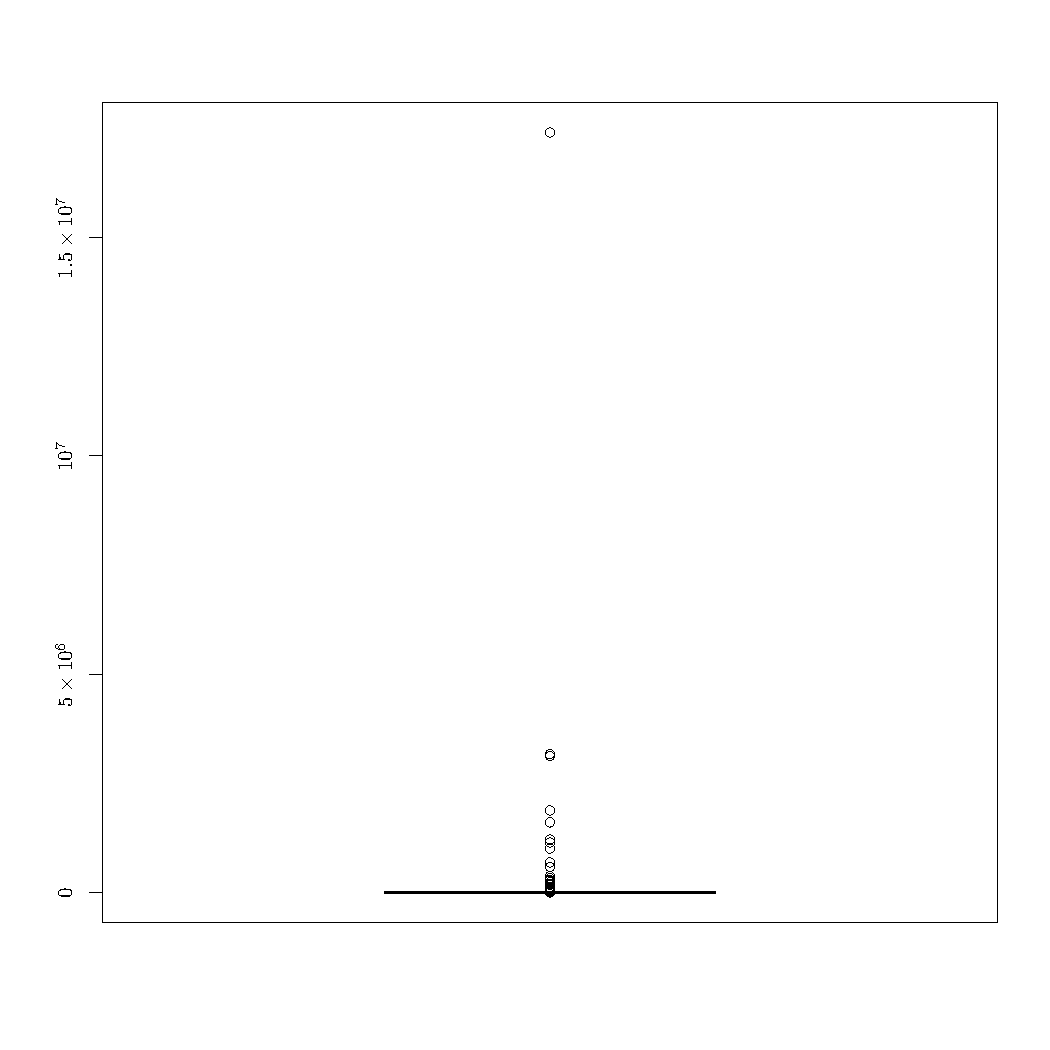
\includegraphics[width=\textwidth]{figures/popuInitialBox.pdf}
        \caption{Boxplot}
        \label{fig:popuInitialBox}
    \end{subfigure}
    \quad
    \begin{subfigure}[b]{0.3\textwidth}
        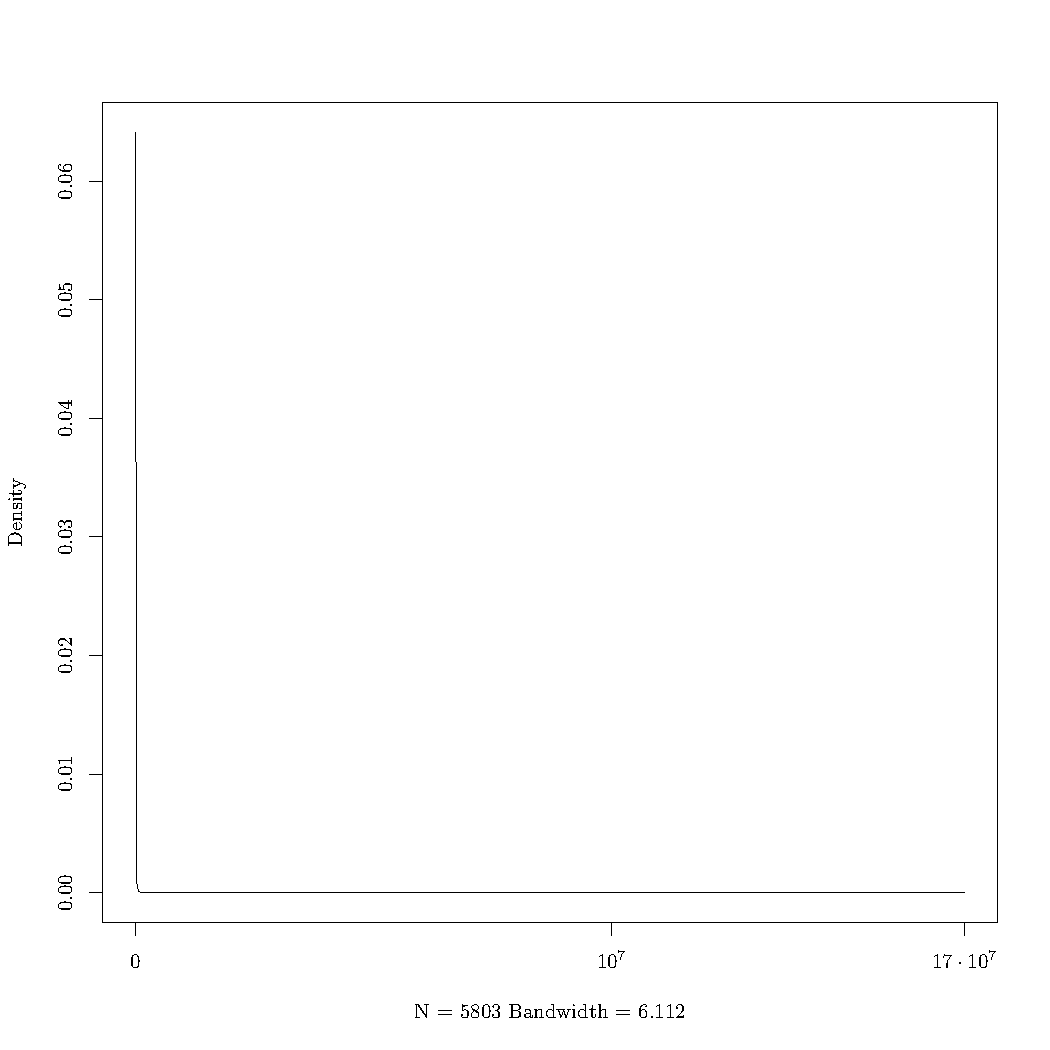
\includegraphics[width=\textwidth]{figures/popuInitialDensity}
        \caption{Density plot}
        \label{fig:popuInitialDensity}
    \end{subfigure}
    \caption{Distribution plots for raw popularity measure.}
\end{figure*}
\begin{figure*}[htb]
    \centering
    \begin{subfigure}[b]{0.3\textwidth}
        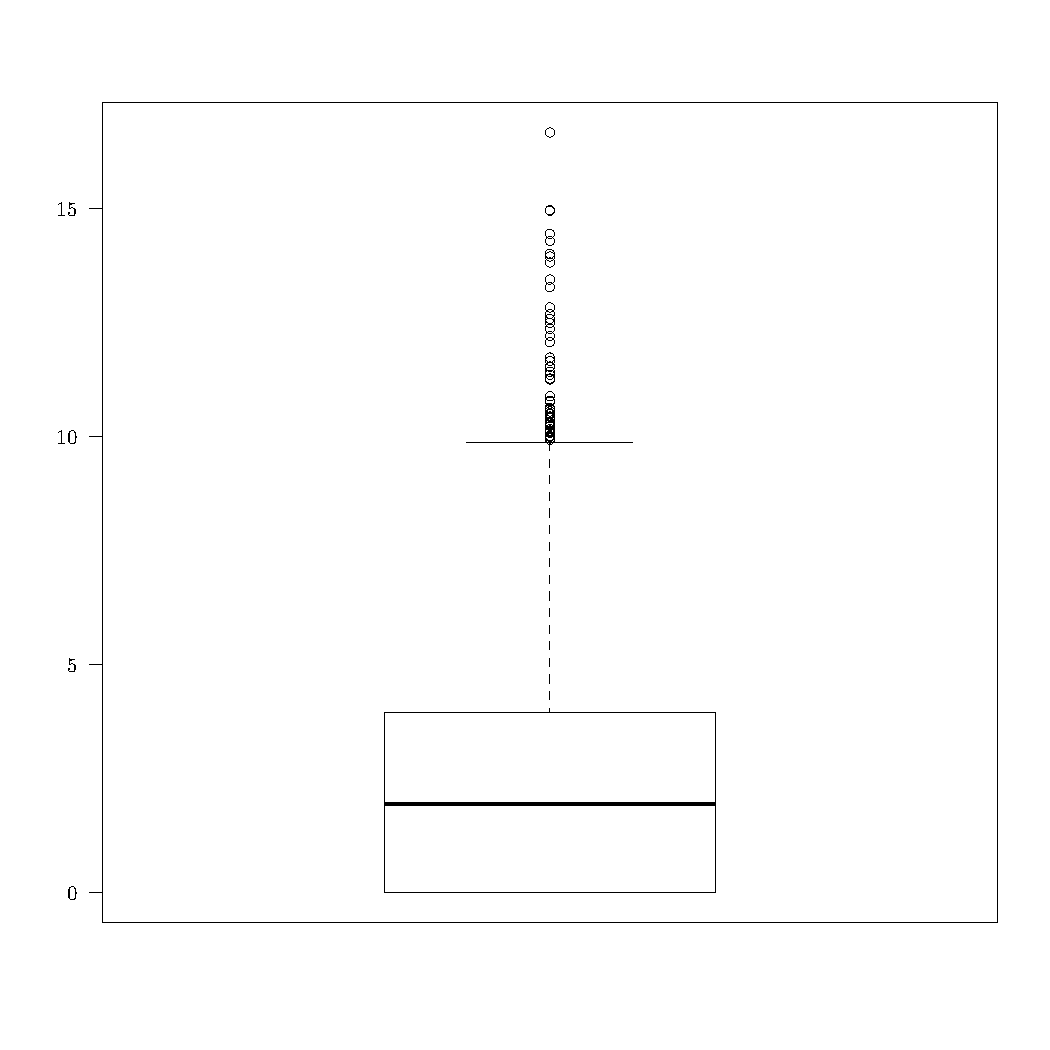
\includegraphics[width=\textwidth]{figures/popuTransformedBox}
        \caption{Boxplot}
        \label{fig:popuTransformedBox}
    \end{subfigure}
    \quad
    \begin{subfigure}[b]{0.3\textwidth}
        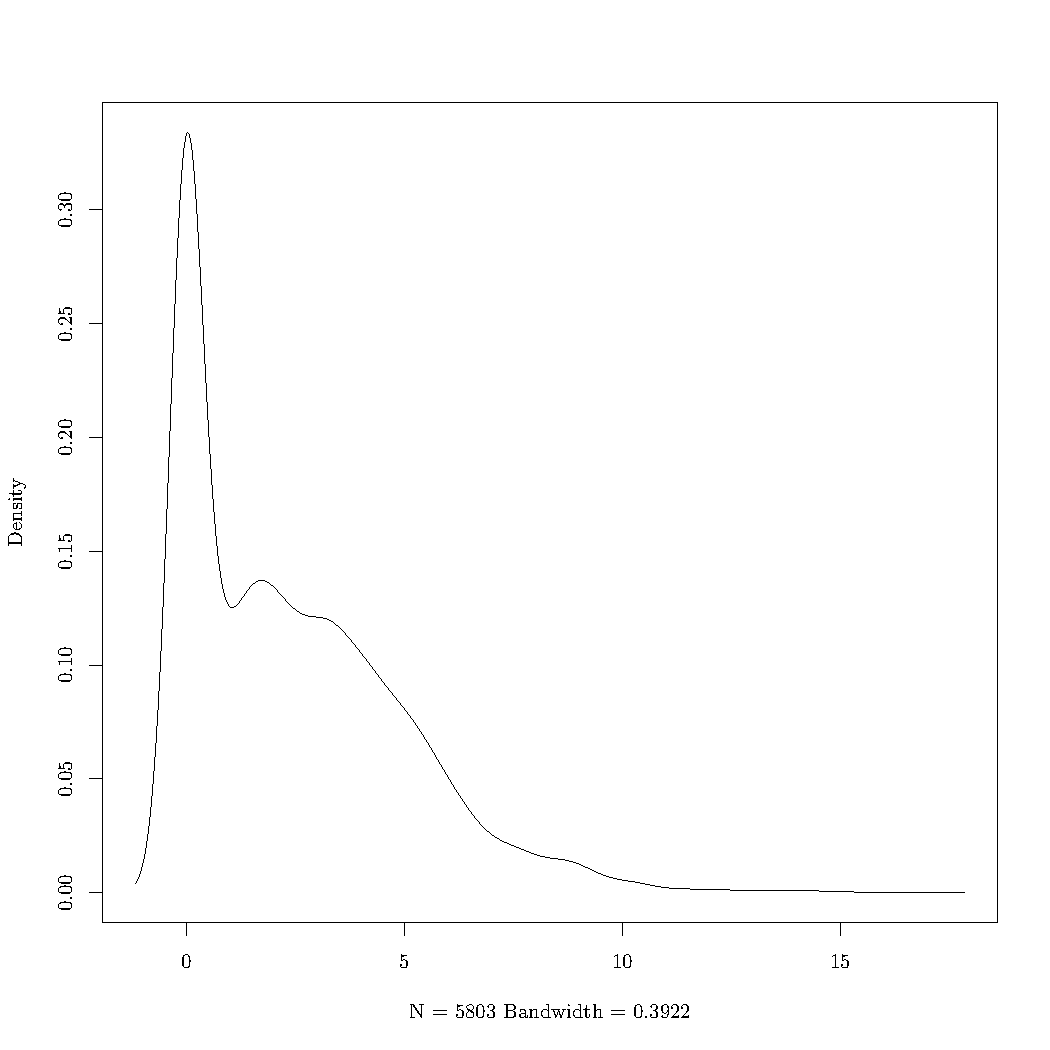
\includegraphics[width=\textwidth]{figures/popuTransformedDensity}
        \caption{Density plot}
        \label{fig:popuTransformedDensity}
    \end{subfigure}
    \caption{Distribution plots for transformed popularity measure.}
\end{figure*}

\subsubsection{Productivity measure}
\label{sssec:productivity}
The productivity measure does have outliers, because searching Google Scholar is always a fuzzy search. For example, searching for "Edgar Allen" gives us a result of 996 publications, which is  probably an overestimate. In order to remove these, we perform standard outlier detection, so we remove all points that lie beyond the extremes of the whiskers. The whiskers are extended to 1.5 times the length of the boxes in the boxplot. A density plot of before and after removing the outliers is shown in Figure~\ref{fig:productivity}.

\begin{figure*}
    \centering
    \begin{subfigure}[b]{0.3\textwidth}
        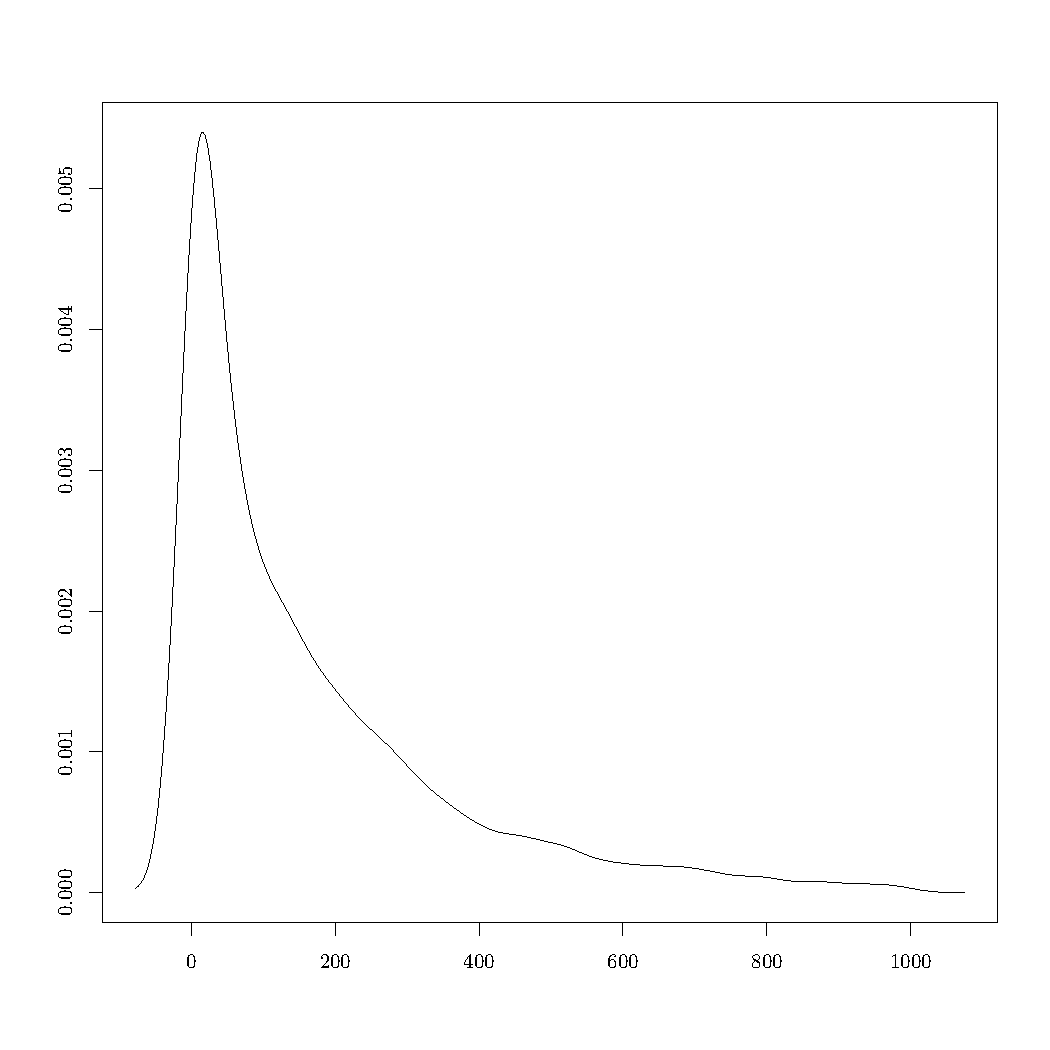
\includegraphics[width=\textwidth]{figures/prodInitialDensity.pdf}
        \caption{Before outlier removal}
        \label{fig:prodInitialDensity}
    \end{subfigure}
    \quad
    \begin{subfigure}[b]{0.3\textwidth}
        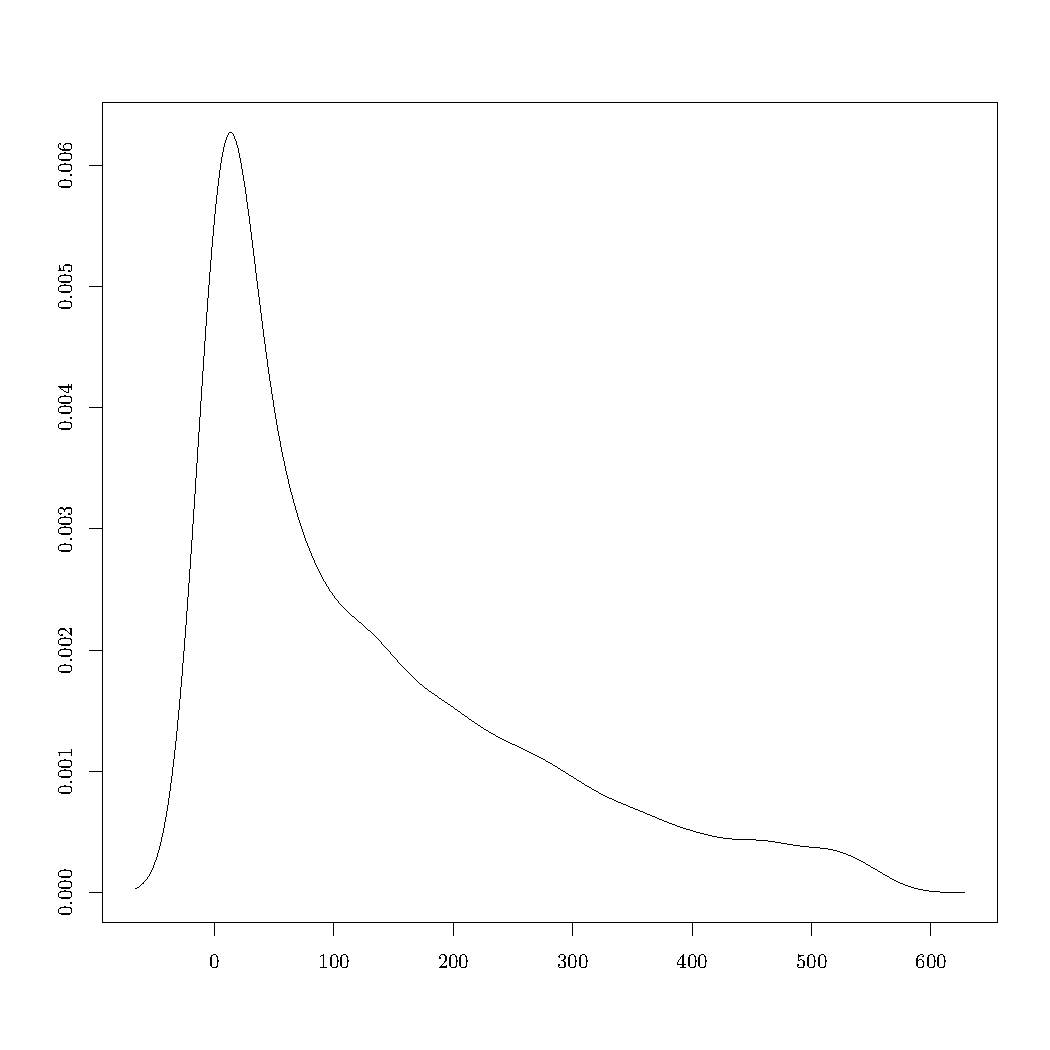
\includegraphics[width=\textwidth]{figures/prodNoOutDensity.pdf}
        \caption{After removing outliers}
        \label{fig:prodNoOutDensity}
    \end{subfigure}
    \caption{Density plots for productivity measure.}
    \label{fig:productivity}
\end{figure*}

After removing outliers, we rescale the data to $[0, 100]$ per category. The resulting means are given below.
\begin{table}[H]
\centering
\begin{tabular}{c|c}
\textbf{\textsc{Nobel}} & \textbf{\textsc{Non-nobel}} \\ \hline
\rule{0pt}{4mm}25.30257&22.79697 \\
\end{tabular}
\end{table}
\noindent Yet again, we test for equality of means and find that they are not equal, however this time only slightly ($p = 0.03971$, only slightly smaller than the default confidence level $0.05$). Note that before removing outliers they were equal according to the test, which supports our decision to remove outliers.

\subsubsection{Resulting training set}
The resulting training set contains 5486 examples, of which 559 positive and 5243 negative.

\subsection{Learning a model}
Not only is the data still relatively fuzzy, the problem that we're facing is a hard one. Creating a model with high precision and recall will probably be impossible. Because of the nature of the test, we want models with a high precision, whereas the recall is less relevant. For example, we do not want lots of politicians to be classified as positive, but when is classified as such, we want that prediction to be as accurate as possible.


\section{Results}
\label{sec:results}

\section{Conclusion}

\section{Future work}

There are still a lot of things that might be interesting to try out, but which we did not do due to time constraints:

\begin{itemize}
    \item It would be interesting to see what happens if we not only consider Nobel Prize winners but also Nobel Prize nominees as positive examples. Nobel Prize nominees are not available on the LoD from Nobelprize.org but can be scraped from the website \cite{nominated}. A problem that this data might pose, is the fact that the names of the nominated people are only made public 50 years after their nomination. This might create a bias in the data, however this is something that should be investigated.
    \item We could also try to include another feature representing which and how many other awards were also won by a person.
    \item For now we only include scientists and economists in our training dataset. We would like to see what happens if we experimented with the other categories of people that can win a Noble Prize as well.
    \item Another thing that is worth looking into is another feature for work productivity. Work productivity seems to have an important relation with winning an award, however it was not even included in our final model. Moreover, our feature of work productivity focusses only on the quantity of work. It would be nice to also have a feature regarding work which focusses on the quality and scientific or political impact of that work (or even better a feature which both captures quantity and quality). An example of such a feature for a scientist is the number of citations he gets per publication.
    
\end{itemize}


% use section* for acknowledgment
\ifCLASSOPTIONcompsoc
  % The Computer Society usually uses the plural form
  \section*{Acknowledgments}
  We would like to thank our supervisors professor Bettina Berendt and Sebastijan Dumancic for their enthousiasm and support.
\else
  % regular IEEE prefers the singular form
  \section*{Acknowledgment}
\fi

% if have a single appendix:
%\appendix[Proof of the Zonklar Equations]
% or
%\appendix  % for no appendix heading
% do not use \section anymore after \appendix, only \section*
% is possibly needed

% use appendices with more than one appendix
% then use \section to start each appendix
% you must declare a \section before using any
% \subsection or using \label (\appendices by itself
% starts a section numbered zero.)
%

% Can use something like this to put references on a page
% by themselves when using endfloat and the captionsoff option.
\ifCLASSOPTIONcaptionsoff
  \newpage
\fi

% trigger a \newpage just before the given reference
% number - used to balance the columns on the last page
% adjust value as needed - may need to be readjusted if
% the document is modified later
%\IEEEtriggeratref{8}
% The "triggered" command can be changed if desired:
%\IEEEtriggercmd{\enlargethispage{-5in}}

% references section

% can use a bibliography generated by BibTeX as a .bbl file
% BibTeX documentation can be easily obtained at:
% http://www.ctan.org/tex-archive/biblio/bibtex/contrib/doc/
% The IEEEtran BibTeX style support page is at:
% http://www.michaelshell.org/tex/ieeetran/bibtex/
%\bibliographystyle{IEEEtran}
% argument is your BibTeX string definitions and bibliography database(s)
%\bibliography{IEEEabrv,../bib/paper}
%
% <OR> manually copy in the resultant .bbl file
% set second argument of \begin to the number of references
% (used to reserve space for the reference number labels box)
\printbibliography


\appendices
%\onecolumn

\clearpage
\section{Discussion on work productivity}
\label{sec:productivity}

Whether we can use different proxy measures for a certain feature is a sensitive issue. For this reason, we here provide a more thorough discussion of the matter. First, we discuss why we have to use different categories of people for building the model and training it. This introduces the problem of having to proxy a feature using  different measures. Next, we discuss why we believe the chosen measures might be a good proxy for the productivity feature. Finally, we give a weakened version of the research question that is now more appropriately answered.

\subsection{Different datasets}

The assignment was to find a research question revolving around the knowledge base, enriched with information from other sources. Because we found an interesting knowledge base on Nobel Prizes, the posed research question wasn't a far fetch. The problem is that in order to build a model on who would win a Nobel Prize, we need positive and negative examples. The positive examples are the Nobel laureates, which come from a pool of scientists. All other scientists naturally serve as negative examples. Since a politician isn't eligible to receive such prize, we can't use them as negative examples. It is thus inevitable to use different examples in the training dataset and the research dataset.

\subsection{Work productivity}

Apart from university rankings and popularity measures, work productivity seems like a reasonable feature to use in order to assess eligibility to receive an award. We reason that hard work will more likely result in making some scientific breakthrough, which increases the chances of someone winning a Nobel Prize. The productivity feature is not trivial to define, however. Furthermore, even if we can define it, all information needed to compute it has to be available for as many training and testing instances as possible. We therefore view all examples as \emph{persons} rather than \emph{scientists} or \emph{politicians}, having certain properties. How we define the work productivity property is the only difference between both datasets. For scientists, the number of publications seems like a decent way of measuring how productive they've been. For politicians, the most resemblant feature would have been the number of legislations they managed to get accepted. This information isn't publicly available, however, so we looked at something else. Coming straight from the ToE knowledge base, the number of speeches at european parliament seemed a good proxy measure. Both are numeric properties which we can normalise to $[0, 100]$.

\subsubsection{Work productivity duality}
An interesting duality exists in both measures. Having a lot of publications over a mediocre amount can be recognised by the model as either a \emph{good} or \emph{bad} property. It can for example mean that someone is just trying to publish a lot of less significant results, while a mediocre amount of significant results might be more important. For speeches the same happens, where a lot of speeches might just as well mean that a politician is only talking, without actually \emph{doing} much. This reinforces our belief that both might be a good proxy for the same feature.

\subsection{Weakened research question}
A more appropriate version of the research question is then
\begin{center}
	\emph{\textbf{\textsc{IF}} the number of publications and the number of speeches in European Parliament are reliable proxies for the work productivity of scientists and politicians respectively \textbf{\textsc{THEN}} which European politicians have a high chance of receiving a Nobel Prize?}
\end{center}


\clearpage
\section{Retrieving data from Google Scholar}
\label{sec:googlescholar}

Retrieving data from Google Scholar is a laborious task. This appendix provides our experience and also our tips on how to scrape Google Scholar. The idea is mimic a user searching stuff trough a browser.


\subsection{Randomised timing.} Halting random amounts of seconds between successive requests vastly increases the number of requests we can do before getting blocked. This happens on two levels: between 15 and 30 seconds between each individual request and another 5 minutes after each 25 requests. 

\subsection{Using cookies.} By performing a search via browser and passing the cookies along with our requests, we trick the server into thinking we are using an actual browser.

\subsection{Using proxies.} We created a script that first scrapes a number of proxies from the internet, verifies if they are not yet blocked by Google Scholar and then performs requests using those proxies. Note that this is very slow, because most random proxies we find are blocked by Google also.


\pagebreak
\section{Linked open data}
\label{sec:lod}
\subsection{Sparql endpoints}
\begin{table}[H]
\centering
\begin{tabular}{l|l}
	\textbf{\textsc{Source}} & \textbf{\textsc{Sparql endpoint}} \\ \hline
	\rule{0pt}{4mm}DBPedia & \texttt{http://dbpedia.org/sparql/} \\
	ToE &  \texttt{http://linkedpolitics.ops.few.vu.nl} \\
	& \texttt{/sparql/} \\
	Nobel Prize & \texttt{http://data.nobelprize.org/sparql}
\end{tabular}
\caption{Overview of used Sparql endpoints.}
\end{table}
\subsection{Difficulties with LoD}
In this section we discuss the difficulties that we experienced with linked open data (LoD). These are worth mentioning because they influenced our results.

\subsubsection{The language barrier}
The great thing about LoD is that it comes in different languages, what means that you have a bigger and a broader information source.
Unfortunately it also brings a lot of difficulties with it.
Not only do the names of people, institutions and other features differ from each other, also the arguments that you give in the queries are sometimes spelled differently.
All these different namings made it more difficult to match the right names with the right features.
That's why we decided to filter everything out that wasn't available in English. One could say that this would create a bias. We decided not to worry about this because the biggest part of LoD is available in English.

\subsubsection{It just doesn't work sometimes}

Apart from the language problem there seem to be Byzantine problems that are really weird. We don't have an explanation nor a solution to address these problems.

\begin{enumerate}
\item \textbf{Links are not broken but queries on them don't work.}\\
Take for example the person Paul R\"ubig. There is an data item about him on DBpedia: \url{http://dbpedia.org/page/Paul\_Rubig}. But if you query this specific resource with the query in Listing~\ref{lst:dbpedia} you will not get any results. 

\item \textbf{\texttt{dati.camera.it} doesn't work at all.}\\
In the ToE database there are lot of reference to the Italian linked open data source \url{dati.camera.it}. Unfortunately none of our queries seem to give any result. Even not for a really simple one, as given in Listing~\ref{lst:dati} and this even though its link \url{http://dati.camera.it/ocd/persona.rdf/p35360} seems to work fine.
\end{enumerate}


\lstinputlisting[language=SQL, caption={Query that doesn't work}, label={lst:dbpedia}, xleftmargin=2em]{queries/dbpedia.rq}
\lstinputlisting[language=SQL, caption={Query that doesn't work on \texttt{dati.camera.it}}, label={lst:dati}, xleftmargin=2em]{queries/dati.rq}



% you can choose not to have a title for an appendix
% if you want by leaving the argument blank
%\section{Google Scholar}


%\section{Source code}
%Appendix two text goes here.
%\lstinputlisting[language=Java, caption=Opdracht 1]{../src/Main.java}
%\lstinputlisting[language=Java, caption=NobelPrice]{../src/NobelPrize.java}
%\lstinputlisting[language=Perl, caption=getRankings.pl]{../scripts/getRankings.pl}

\end{document}
